\documentclass[12pt]{article}
\usepackage{amsmath}
\usepackage{kotex}
\usepackage{graphicx}
\usepackage{hyperref}
\usepackage[framemethod=tikz]{mdframed}
\title{Assignment01}
\author{20124602 이승준}
\date{Sep.21.2018}
\begin{document}
  \maketitle
  \section[시작]{git 이란?}
  	\ Git이란 오픈 소프트웨어코드 저장소의 대표적인 하나이며, git덕분에 오픈소스 업계가 큰 발전을 이루었다고 하는것은 과언이 아니다. git의 작업서버의 전체 기록과 각 기록을 추적할 수 있는 정보를 포함하고 있어서, 프로그래머가 수정하기전의 코드를 쉽게 열람이 가능하고, 이를 개인 컴퓨터에 간단한 명령어를 통해 카피 할 수 있다. github를 통하여 git으로 사람들이 공유하고있는 코드를 실체화 할 수 있다.

    
  \subsection{ \textit{\href{https://git-scm.com/download/win}{github}} 가입하기}
  \ git을 사용하기 위해선 우선 자신만의 github가 필요하다. 	
  	가입은 간단하게 자신이 사용하고 있는 이메일 주소만 입력하면 가입이 완성이 될것이다.
   \begin{figure}[!hbp]
   	\centering   
   	\label{github main}
   	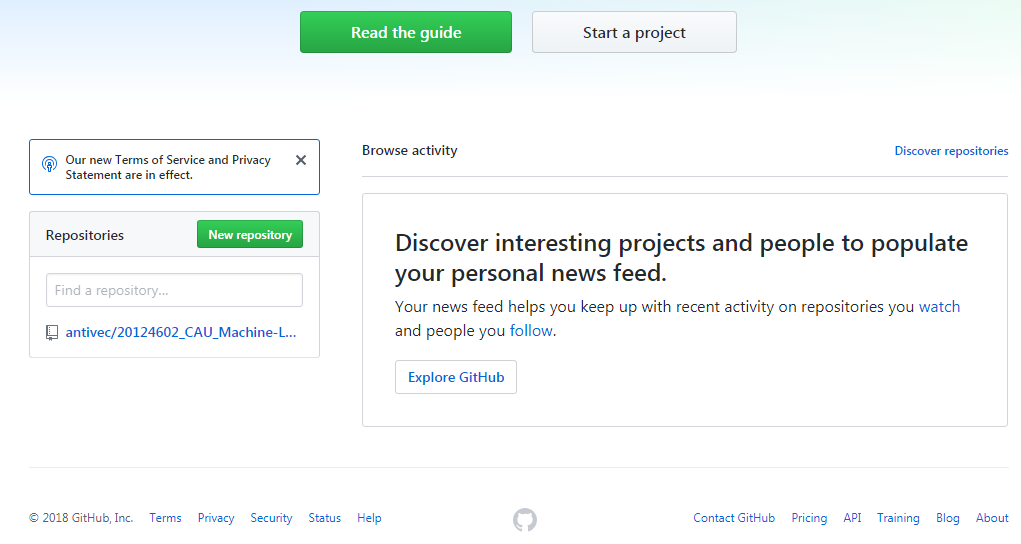
\includegraphics[width=0.75\textwidth]{main_github}
   	\caption{github 메인화면}
   \end{figure}
	\subsection{프로젝트 시작하기}
  	github에 개인용 또는 팀용 프로젝트를 시작하려면 다음과 같은 간단한 과정 걸쳐야 한다.
  	\begin{mdframed}[
  		linecolor= black,
  		roundcorner=10pt,
  		innertopmargin =\topskip,
  		leftmargin = 0.5cm,
  		rightmargin = 0.5cm,
  		frametitleaboveskip = 0.5pt,
  		frametitlerulewidth = 0.5pt,
  		frametitlealignment =,
  		frametitlebackgroundcolor = yellow,			
  		frametitle = {githhub 가입하기}	]
  		\begin{enumerate}
  			\item Start a Project 클릭
  			
  			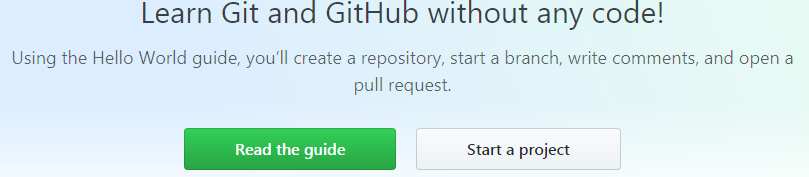
\includegraphics[width=0.75\textwidth]{start}
  			\item Repository name에 프로젝트의 이름 및 설명 입력
  			
  			 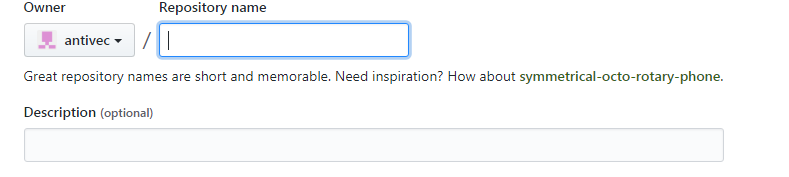
\includegraphics[width=0.75\textwidth]{owner}
  			\item 프로젝트의 공개여부와 README.md 파일 생성 유무를 설정  			
  			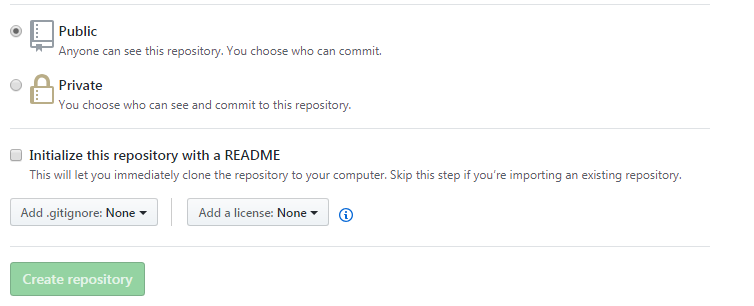
\includegraphics[width=0.75\textwidth]{publc}
  		\end{enumerate}  		
  	\end{mdframed} 
  최종적으로 다음과 같은 프로젝트가 공간이 생길것이다.\footnote{\href{https://github.com/antivec/20124602_CAU_Machine-Learning}{https://github.com/antivec/20124602 CAU Machine-Learning}}  
  \begin{figure}[!hbp] 
  	\label{create_repository}
  	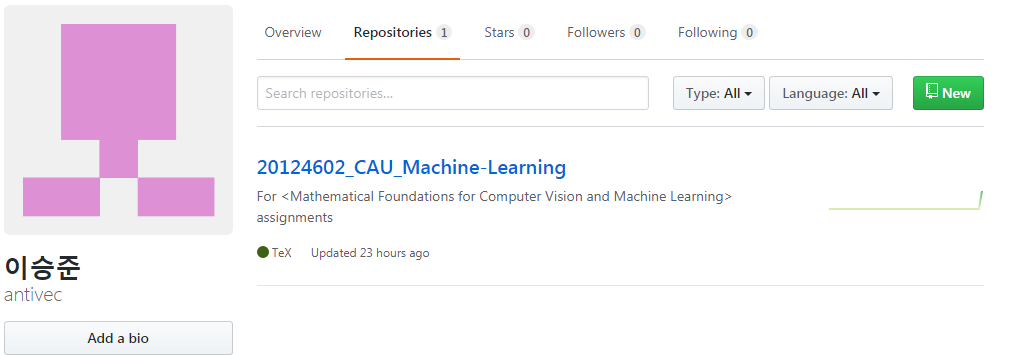
\includegraphics[width=0.65\textwidth]{create_repository}
  	\caption{\textsl{repository 생성후}}
  \end{figure}

\section{git 활용하기}
	\textit{\href{https://git-scm.com/download/win}{git홈페이지}}에 들어가 git을 설치하게 되면 다음과 같은(figure3) cmd창을 실행할 수 있다
	\begin{figure}		
		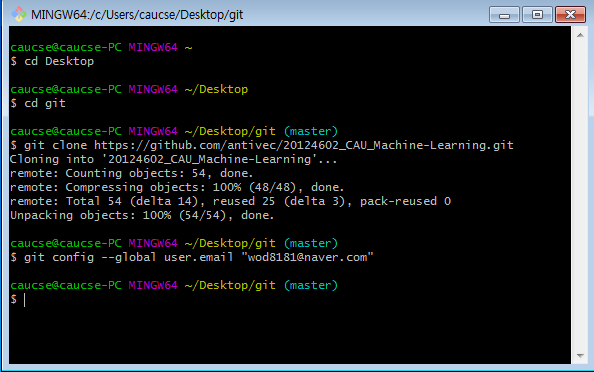
\includegraphics[width=0.75\textwidth]{git_cmd}
		\caption{github 메인화면}
	\end{figure}

	
	기본적인 명령어는 windows cmd와 많이 흡사하다.
	이를 통해 OS환경에 구속되지 않고 프로젝트를 업로드하거나 local로 다운로드 받는것이 가능하다.
	
	우선적으로 git에서 프로젝트를 다운받거나 업로드를 하기 위해선 해당 폴더에 git환경을 조성해야한다.명령어는 다음과 같다.
	\begin{mdframed}[
		linecolor= black,
		roundcorner=10pt,
		innertopmargin =\topskip,
		leftmargin = 0.5cm,
		rightmargin = 0.5cm,
		frametitleaboveskip = 0.5pt,
		frametitlerulewidth = 0.5pt,
		frametitlealignment =,
		frametitlebackgroundcolor = yellow,			
		frametitle = {git환경 설정하기}	]
		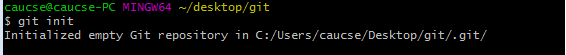
\includegraphics[width=\textwidth]{git_init}
		git init		
	\end{mdframed}
	해당 폴더의 git환경이 설정이 완료가 되면 해당 폴더의 사용자의 프로필을 설정하여야 한다
	\begin{mdframed}[
		linecolor= black,
		roundcorner=10pt,
		innertopmargin =\topskip,
		leftmargin = 0.5cm,
		rightmargin = 0.5cm,
		frametitleaboveskip = 0.5pt,
		frametitlerulewidth = 0.5pt,
		frametitlealignment =,
		frametitlebackgroundcolor = yellow,			
		frametitle = {git프로필 설정하기}	]
		\begin{enumerate}
			\item git config --global user.name = "" \footnote{이름 설정}	
			\item git config --global user.email = ""	\footnote{이메일 설정}

		\end{enumerate}  		
	\end{mdframed}
	\subsection{github로부터 프로젝트 받기}
	앞선 그림처럼 git환경 초기화가 성공했을경우, githhub에 올린 프로젝트를 다음과 같은 명령어로 해당 폴더에 local로 받을수 있다
		\begin{mdframed}[
			linecolor= black,
			roundcorner=10pt,
			innertopmargin =\topskip,
			leftmargin = 0.5cm,
			rightmargin = 0.5cm,
			frametitleaboveskip = 0.5pt,
			frametitlerulewidth = 0.5pt,
			frametitlealignment =,
			frametitlebackgroundcolor = yellow,			
			frametitle = {git으로부터 프로젝트 받기}	]
			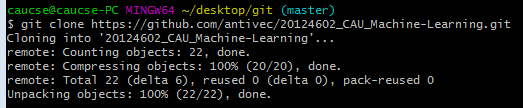
\includegraphics[width=\textwidth]{git_clone}
			- git clone  \href{https://github.com/antivec/20124602_CAU_Machine-Learning}{다운받고자 하는 github의 주소}
			
			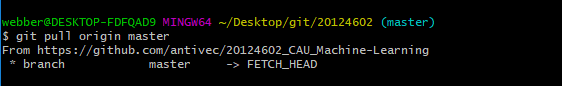
\includegraphics[width=\textwidth]{git_pull}
			git clone으로 프로젝트를 받은후에는 git pull로 local저장소에 수정된 코드를 얻어 올 수 있다.
			- git pull
		\end{mdframed}
		
		\subsection{local에서 수정한 코드를 github에 업로드 하기}
	local에서 수정한 코드를 github에 업로드를 하기 위해서는 다음과 같은 과정이 필요하다.
	\begin{mdframed}[
		linecolor= black,
		roundcorner=10pt,
		innertopmargin =\topskip,
		leftmargin = 0.5cm,
		rightmargin = 0.5cm,
		frametitleaboveskip = 0.5pt,
		frametitlerulewidth = 0.5pt,
		frametitlealignment =,
		frametitlebackgroundcolor = yellow,			
		frametitle = {githhub에 수정된 파일 올리기}	]
		\begin{enumerate}
			\item git add . //변동이 생긴 모든 파일을 github 업로드 한다 \footnote{add뒤에 파일명을 입력하면, 해당 변동된 파일만 업로드한다}
			
			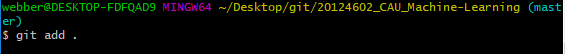
\includegraphics[width=0.75\textwidth]{add}
			
			\item git commit -m "" // 업로드한 변동이 생긴 파일에 description을 생성한다			
			
			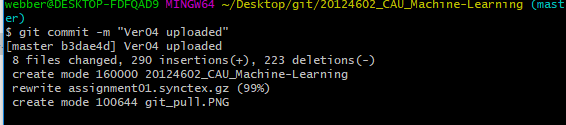
\includegraphics[width=0.75\textwidth]{commit}
			
			\item git push //github에 등록한다
			
			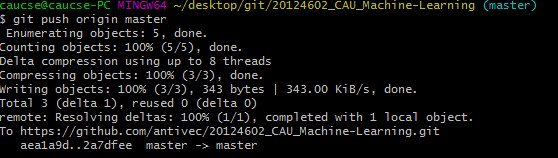
\includegraphics[width=0.75\textwidth]{push}
			
			\item 성공적으로 업로드가 되면 다음과 같이 업로드 된다
			
			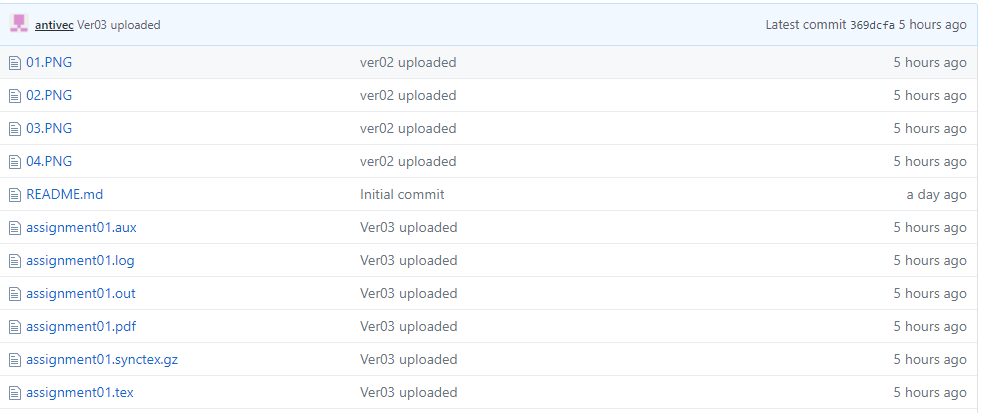
\includegraphics[width=0.75\textwidth]{result}
		\end{enumerate}  		
	\end{mdframed} 
  %	\href{https://github.com/antivec/20124602_CAU_Machine-Learning}{github 주소}
  % This is a comment; it will not be shown in the final output.
  % The following shows a little of the typesetting power of LaTeX:


\end{document}

  $ pdflatex assignment01.tex